\documentclass[11pt,psfig]{article}
\usepackage{epsfig}
\usepackage{times}
\usepackage{amssymb}
\usepackage{float}

\newcount\refno\refno=1
\def\ref{\the\refno \global\advance\refno by 1}
\def\ux{\underline{x}}
\def\uw{\underline{w}}
\def\bw{\underline{w}}
\def\ut{\underline{\theta}}
\def\umu{\underline{\mu}} 
\def\bmu{\underline{\mu}} 
\def\be{p_e^*}
\newcount\eqnumber\eqnumber=1
\def\eq{\the \eqnumber \global\advance\eqnumber by 1}
\def\eqs{\eq}
\def\eqn{\eqno(\eq)}

 \pagestyle{empty}
\def\baselinestretch{1.1}
\topmargin1in \headsep0.3in
\topmargin0in \oddsidemargin0in \textwidth6.5in \textheight8.5in
\begin{document}
\setlength{\parskip}{1.2ex plus0.3ex minus 0.3ex}


\thispagestyle{empty} \pagestyle{myheadings} \markright{G}



\title{CS 266 Homework 3}
\author{Zachary DeStefano, PhD Student, 15247592}
\date{Due Date: April 24}

\maketitle

\vfill\eject

\section*{Problem 3.11}

Give an efficient algorithm to determine whether a polygon P with n
vertices is monotone with respect to some line, not necessarily a horizontal
or vertical one.\\
\\
For this algorithm, we will use a version of the plane sweep algorithm. We will sweep a horizontal line at each vertex and if the intersection is more than just two points, a line segment, or empty, then it is not monotone. \\
\\
Here is the algorithm:\\
1. Sort the vertices by y-coordinate\\
2. Make an interval tree data structure for the $y_{min}$ and $y_{max}$ coordinates of each of the segments. \\
\begin{verbatim}
http://en.wikipedia.org/wiki/Interval_tree#Centered_interval_tree
\end{verbatim}
3. For each vertex v, do the following:\\
- Sweep a horizontal line at its y-coordinate\\
- If the number of other segments or points with that same y-coordinate is more than 1\\
or there is at least one other intersection but v is part of a horizontal segment, then\\
declare that P is not monotone and exit.\\
(TODO: Detail the data structure to be used here)\\
4. If P has not been declared non-monotone, then P is monotone\\
\\
Correctness:\\
All the parts where the it will not be polygon will be at event points, which are the vertices. (TODO: Prove this)\\
\\
Running time: \\
Step 1 will take O(n log n) time. \\
Constructing an interval tree for Step 2 is O(n log n) time. \\
There are n vertices to test in the worst case. \\
For each vertex, the query will take O($log n + 2$) time since we are requesting 2 results. \\
Thus the total running time ends up being O(n log n)\\

\newpage

\section*{Problem 3.14}

Given a simple polygon P with n vertices and a point p inside it, show
how to compute the region inside P that is visible from p.\\
\\
In the following figure, the visible region is the triangles with an X inside them. \\
\begin{figure}[H]
\centering
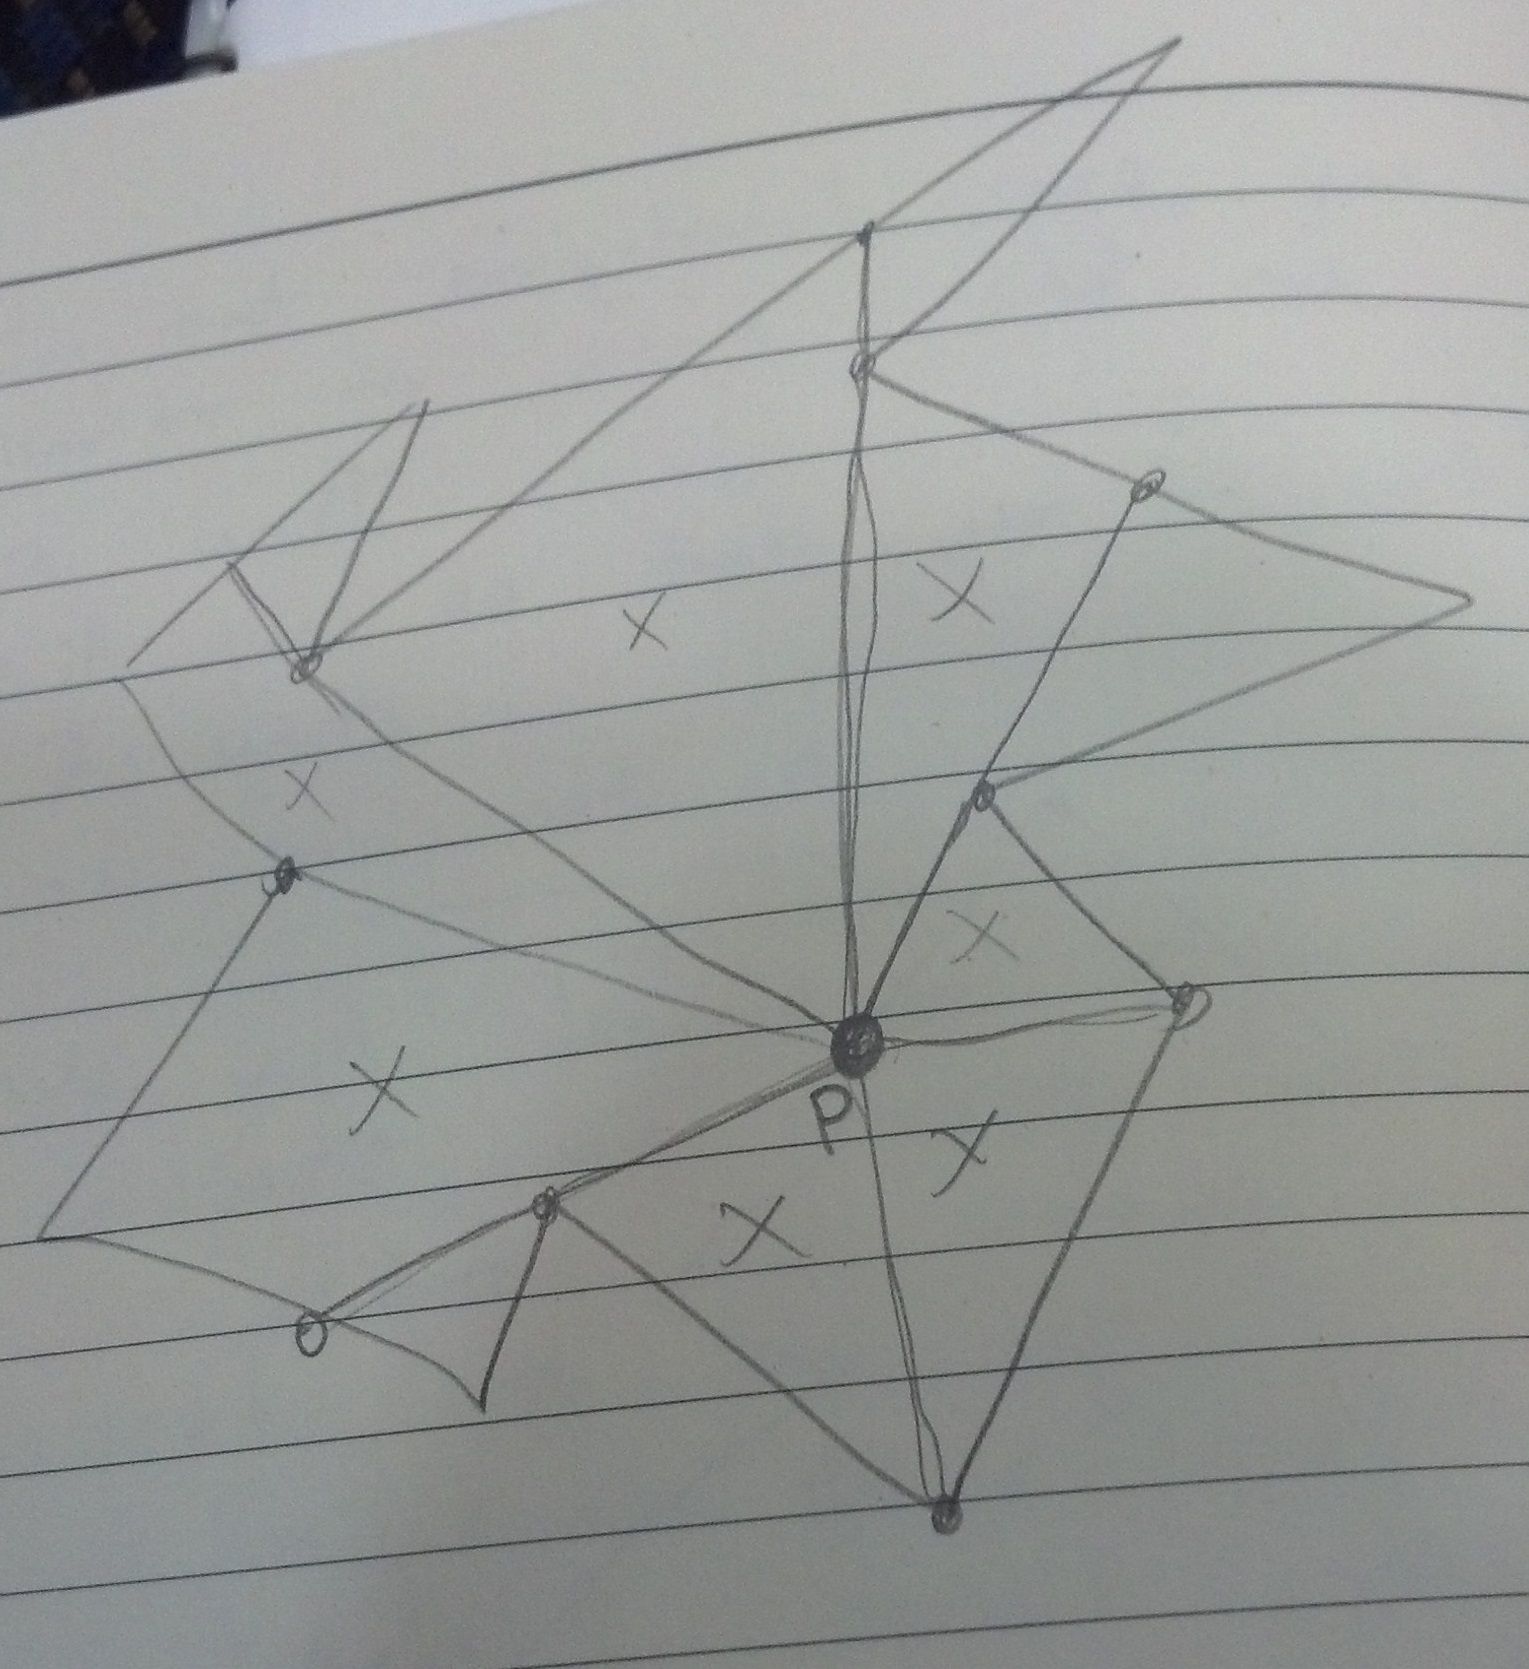
\includegraphics[height=4in]{visible_regions.jpg}
\caption{Parts of polygon visible from point p}
\end{figure}

The following procedure will be used:\\
For each vertex v with unobstructed view of p:\\
- Construct line segment from p, then passing through v, and ending at the next line segment in that direction. \\
- All the triangles that have just been constructed that are around p are the visible region. 

\newpage

\section*{Problem 15.2}

Algorithm VISIBILITYGRAPH calls algorithm VISIBLEVERTICES with
each obstacle vertex. VISIBLEVERTICES sorts all vertices around its
input point. This means that n cyclic sortings are done, one around each
obstacle vertex. In this chapter we simply did every sort in O(nlogn)
time, leading to O(n2 logn)time for all sortings. Show that this can be
improved to O(n2) time using dualization (see Chapter 8). Does this
improve the running time of VISIBILITYGRAPH?

\newpage

\section*{Problem 15.4}

What is the maximal number of shortest paths connecting two fixed
points among a set of n triangles in the plane?

\end{document}








